\documentclass[]{article}
\usepackage{lmodern}
\usepackage{amssymb,amsmath}
\usepackage{ifxetex,ifluatex}
\usepackage{fixltx2e} % provides \textsubscript
\ifnum 0\ifxetex 1\fi\ifluatex 1\fi=0 % if pdftex
  \usepackage[T1]{fontenc}
  \usepackage[utf8]{inputenc}
\else % if luatex or xelatex
  \ifxetex
    \usepackage{mathspec}
  \else
    \usepackage{fontspec}
  \fi
  \defaultfontfeatures{Ligatures=TeX,Scale=MatchLowercase}
\fi
% use upquote if available, for straight quotes in verbatim environments
\IfFileExists{upquote.sty}{\usepackage{upquote}}{}
% use microtype if available
\IfFileExists{microtype.sty}{%
\usepackage{microtype}
\UseMicrotypeSet[protrusion]{basicmath} % disable protrusion for tt fonts
}{}
\usepackage[margin=1in]{geometry}
\usepackage{hyperref}
\hypersetup{unicode=true,
            pdftitle={Analyses\_and\_Plots},
            pdfauthor={Austin Hammer},
            pdfborder={0 0 0},
            breaklinks=true}
\urlstyle{same}  % don't use monospace font for urls
\usepackage{color}
\usepackage{fancyvrb}
\newcommand{\VerbBar}{|}
\newcommand{\VERB}{\Verb[commandchars=\\\{\}]}
\DefineVerbatimEnvironment{Highlighting}{Verbatim}{commandchars=\\\{\}}
% Add ',fontsize=\small' for more characters per line
\usepackage{framed}
\definecolor{shadecolor}{RGB}{248,248,248}
\newenvironment{Shaded}{\begin{snugshade}}{\end{snugshade}}
\newcommand{\AlertTok}[1]{\textcolor[rgb]{0.94,0.16,0.16}{#1}}
\newcommand{\AnnotationTok}[1]{\textcolor[rgb]{0.56,0.35,0.01}{\textbf{\textit{#1}}}}
\newcommand{\AttributeTok}[1]{\textcolor[rgb]{0.77,0.63,0.00}{#1}}
\newcommand{\BaseNTok}[1]{\textcolor[rgb]{0.00,0.00,0.81}{#1}}
\newcommand{\BuiltInTok}[1]{#1}
\newcommand{\CharTok}[1]{\textcolor[rgb]{0.31,0.60,0.02}{#1}}
\newcommand{\CommentTok}[1]{\textcolor[rgb]{0.56,0.35,0.01}{\textit{#1}}}
\newcommand{\CommentVarTok}[1]{\textcolor[rgb]{0.56,0.35,0.01}{\textbf{\textit{#1}}}}
\newcommand{\ConstantTok}[1]{\textcolor[rgb]{0.00,0.00,0.00}{#1}}
\newcommand{\ControlFlowTok}[1]{\textcolor[rgb]{0.13,0.29,0.53}{\textbf{#1}}}
\newcommand{\DataTypeTok}[1]{\textcolor[rgb]{0.13,0.29,0.53}{#1}}
\newcommand{\DecValTok}[1]{\textcolor[rgb]{0.00,0.00,0.81}{#1}}
\newcommand{\DocumentationTok}[1]{\textcolor[rgb]{0.56,0.35,0.01}{\textbf{\textit{#1}}}}
\newcommand{\ErrorTok}[1]{\textcolor[rgb]{0.64,0.00,0.00}{\textbf{#1}}}
\newcommand{\ExtensionTok}[1]{#1}
\newcommand{\FloatTok}[1]{\textcolor[rgb]{0.00,0.00,0.81}{#1}}
\newcommand{\FunctionTok}[1]{\textcolor[rgb]{0.00,0.00,0.00}{#1}}
\newcommand{\ImportTok}[1]{#1}
\newcommand{\InformationTok}[1]{\textcolor[rgb]{0.56,0.35,0.01}{\textbf{\textit{#1}}}}
\newcommand{\KeywordTok}[1]{\textcolor[rgb]{0.13,0.29,0.53}{\textbf{#1}}}
\newcommand{\NormalTok}[1]{#1}
\newcommand{\OperatorTok}[1]{\textcolor[rgb]{0.81,0.36,0.00}{\textbf{#1}}}
\newcommand{\OtherTok}[1]{\textcolor[rgb]{0.56,0.35,0.01}{#1}}
\newcommand{\PreprocessorTok}[1]{\textcolor[rgb]{0.56,0.35,0.01}{\textit{#1}}}
\newcommand{\RegionMarkerTok}[1]{#1}
\newcommand{\SpecialCharTok}[1]{\textcolor[rgb]{0.00,0.00,0.00}{#1}}
\newcommand{\SpecialStringTok}[1]{\textcolor[rgb]{0.31,0.60,0.02}{#1}}
\newcommand{\StringTok}[1]{\textcolor[rgb]{0.31,0.60,0.02}{#1}}
\newcommand{\VariableTok}[1]{\textcolor[rgb]{0.00,0.00,0.00}{#1}}
\newcommand{\VerbatimStringTok}[1]{\textcolor[rgb]{0.31,0.60,0.02}{#1}}
\newcommand{\WarningTok}[1]{\textcolor[rgb]{0.56,0.35,0.01}{\textbf{\textit{#1}}}}
\usepackage{graphicx,grffile}
\makeatletter
\def\maxwidth{\ifdim\Gin@nat@width>\linewidth\linewidth\else\Gin@nat@width\fi}
\def\maxheight{\ifdim\Gin@nat@height>\textheight\textheight\else\Gin@nat@height\fi}
\makeatother
% Scale images if necessary, so that they will not overflow the page
% margins by default, and it is still possible to overwrite the defaults
% using explicit options in \includegraphics[width, height, ...]{}
\setkeys{Gin}{width=\maxwidth,height=\maxheight,keepaspectratio}
\IfFileExists{parskip.sty}{%
\usepackage{parskip}
}{% else
\setlength{\parindent}{0pt}
\setlength{\parskip}{6pt plus 2pt minus 1pt}
}
\setlength{\emergencystretch}{3em}  % prevent overfull lines
\providecommand{\tightlist}{%
  \setlength{\itemsep}{0pt}\setlength{\parskip}{0pt}}
\setcounter{secnumdepth}{0}
% Redefines (sub)paragraphs to behave more like sections
\ifx\paragraph\undefined\else
\let\oldparagraph\paragraph
\renewcommand{\paragraph}[1]{\oldparagraph{#1}\mbox{}}
\fi
\ifx\subparagraph\undefined\else
\let\oldsubparagraph\subparagraph
\renewcommand{\subparagraph}[1]{\oldsubparagraph{#1}\mbox{}}
\fi

%%% Use protect on footnotes to avoid problems with footnotes in titles
\let\rmarkdownfootnote\footnote%
\def\footnote{\protect\rmarkdownfootnote}

%%% Change title format to be more compact
\usepackage{titling}

% Create subtitle command for use in maketitle
\providecommand{\subtitle}[1]{
  \posttitle{
    \begin{center}\large#1\end{center}
    }
}

\setlength{\droptitle}{-2em}

  \title{Analyses\_and\_Plots}
    \pretitle{\vspace{\droptitle}\centering\huge}
  \posttitle{\par}
    \author{Austin Hammer}
    \preauthor{\centering\large\emph}
  \postauthor{\par}
      \predate{\centering\large\emph}
  \postdate{\par}
    \date{11/5/2019}


\begin{document}
\maketitle

library(``ggplot2'') library(``dplyr'') library(``vegan'')
library(``DESeq2'') library(``knitr'')

\begin{verbatim}
## Warning in estimate_richness(physeq1, split = TRUE, measures = c("Shannon")): The data you have provided does not have
## any singletons. This is highly suspicious. Results of richness
## estimates (for example) are probably unreliable, or wrong, if you have already
## trimmed low-abundance taxa from the data.
## 
## We recommended that you find the un-trimmed data and retry.
\end{verbatim}

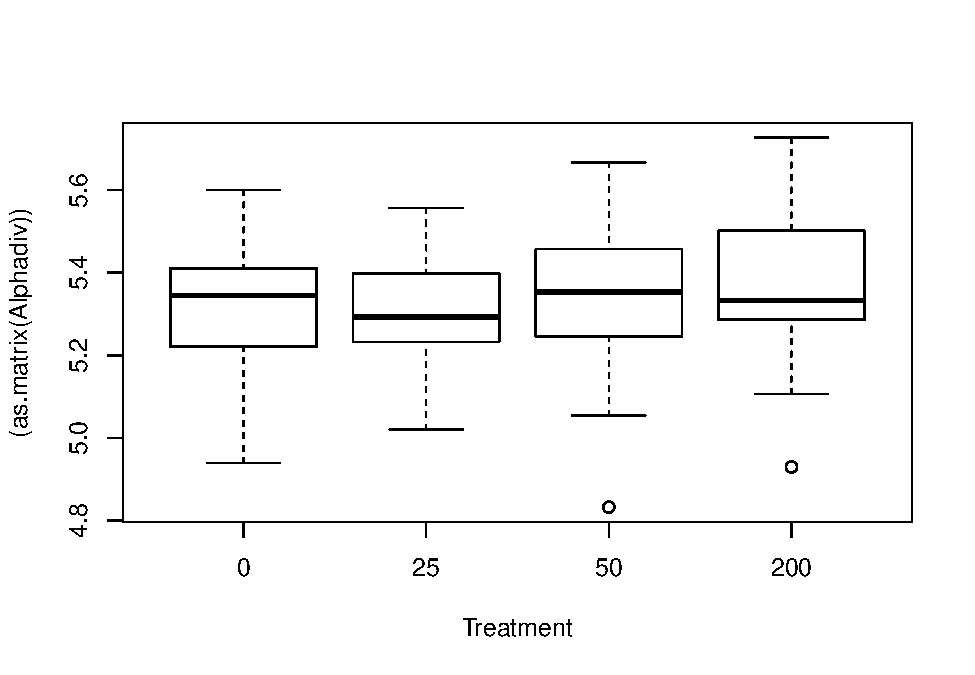
\includegraphics{Analyses_and_Plots_files/figure-latex/alphadiv-1.pdf}
\includegraphics{Analyses_and_Plots_files/figure-latex/alphadiv-2.pdf}
\includegraphics{Analyses_and_Plots_files/figure-latex/alphadiv-3.pdf}
\includegraphics{Analyses_and_Plots_files/figure-latex/alphadiv-4.pdf}
\includegraphics{Analyses_and_Plots_files/figure-latex/alphadiv-5.pdf}

\begin{verbatim}
## Analysis of Variance Table
## 
## Response: as.matrix(Alphadiv)
##           Df  Sum Sq  Mean Sq F value Pr(>F)
## Treatment  1 0.05269 0.052686  2.2074 0.1407
## Residuals 95 2.26745 0.023868
\end{verbatim}

\begin{verbatim}
## 
##  Kendall's rank correlation tau
## 
## data:  anova_df$FSTTimeImmobile and (as.matrix(anova_df$Alphadiv))
## z = 2.0181, p-value = 0.04359
## alternative hypothesis: true tau is not equal to 0
## sample estimates:
##       tau 
## 0.1405853
\end{verbatim}

\begin{verbatim}
## Loading required package: permute
\end{verbatim}

\begin{verbatim}
## Loading required package: lattice
\end{verbatim}

\begin{verbatim}
## This is vegan 2.5-5
\end{verbatim}

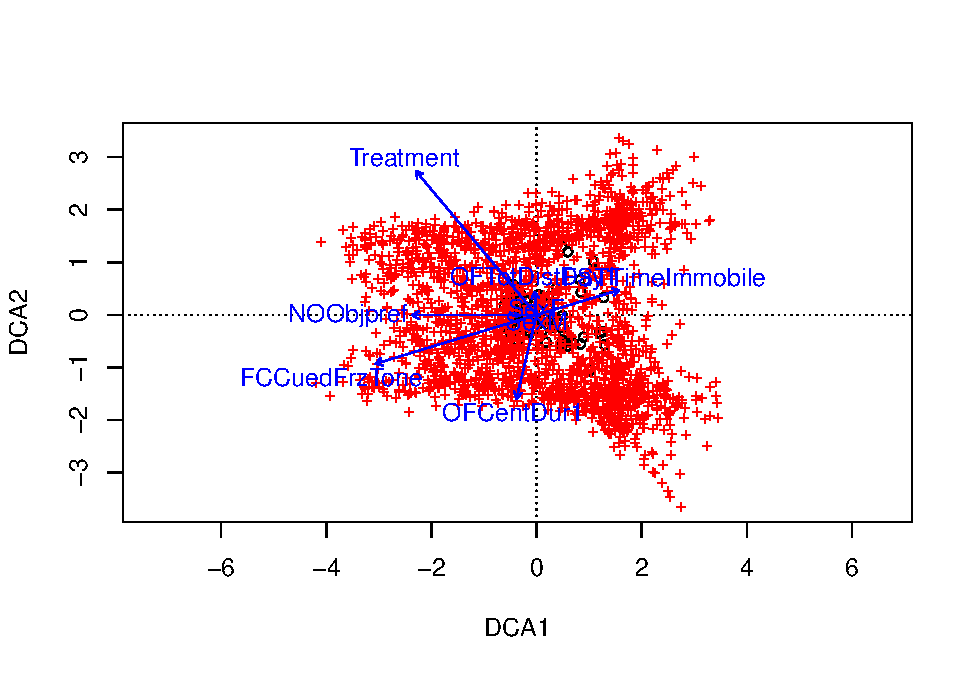
\includegraphics{Analyses_and_Plots_files/figure-latex/enfit-1.pdf}

\begin{verbatim}
## Warning in decorana(data.frame(otu_table(physeq1))): some species were
## removed because they were missing in the data
\end{verbatim}

\includegraphics{Analyses_and_Plots_files/figure-latex/enfit-2.pdf}

\begin{verbatim}
## Square root transformation
## Wisconsin double standardization
## Run 0 stress 0.2329333 
## Run 1 stress 0.2273835 
## ... New best solution
## ... Procrustes: rmse 0.0466619  max resid 0.4289286 
## Run 2 stress 0.2465755 
## Run 3 stress 0.2384712 
## Run 4 stress 0.2322097 
## Run 5 stress 0.242879 
## Run 6 stress 0.2272464 
## ... New best solution
## ... Procrustes: rmse 0.004871792  max resid 0.03189437 
## Run 7 stress 0.2401365 
## Run 8 stress 0.2281104 
## Run 9 stress 0.232136 
## Run 10 stress 0.2323704 
## Run 11 stress 0.232757 
## Run 12 stress 0.2313536 
## Run 13 stress 0.2435032 
## Run 14 stress 0.2327983 
## Run 15 stress 0.2389518 
## Run 16 stress 0.2301668 
## Run 17 stress 0.23482 
## Run 18 stress 0.2307502 
## Run 19 stress 0.2282109 
## Run 20 stress 0.2325069 
## *** No convergence -- monoMDS stopping criteria:
##     20: stress ratio > sratmax
\end{verbatim}

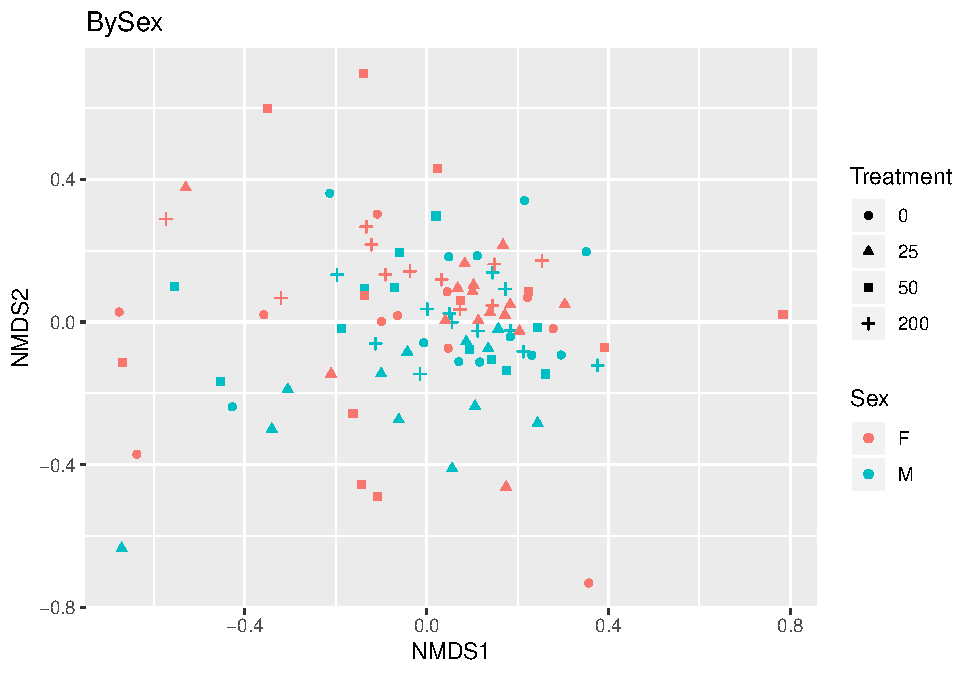
\includegraphics{Analyses_and_Plots_files/figure-latex/bray_by_Sex_Treatment-1.pdf}
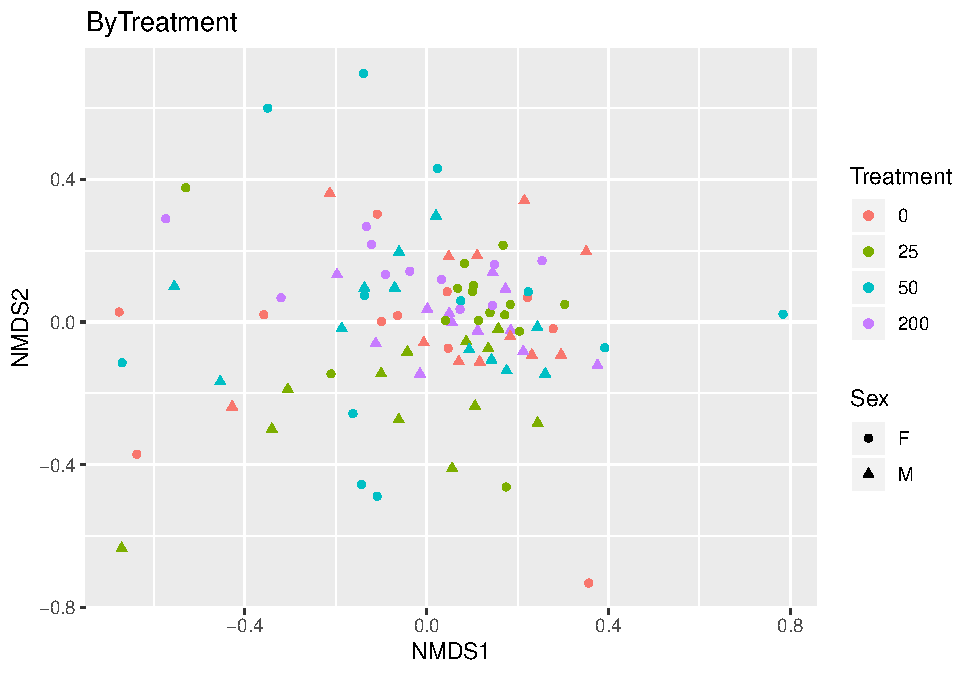
\includegraphics{Analyses_and_Plots_files/figure-latex/bray_by_Sex_Treatment-2.pdf}
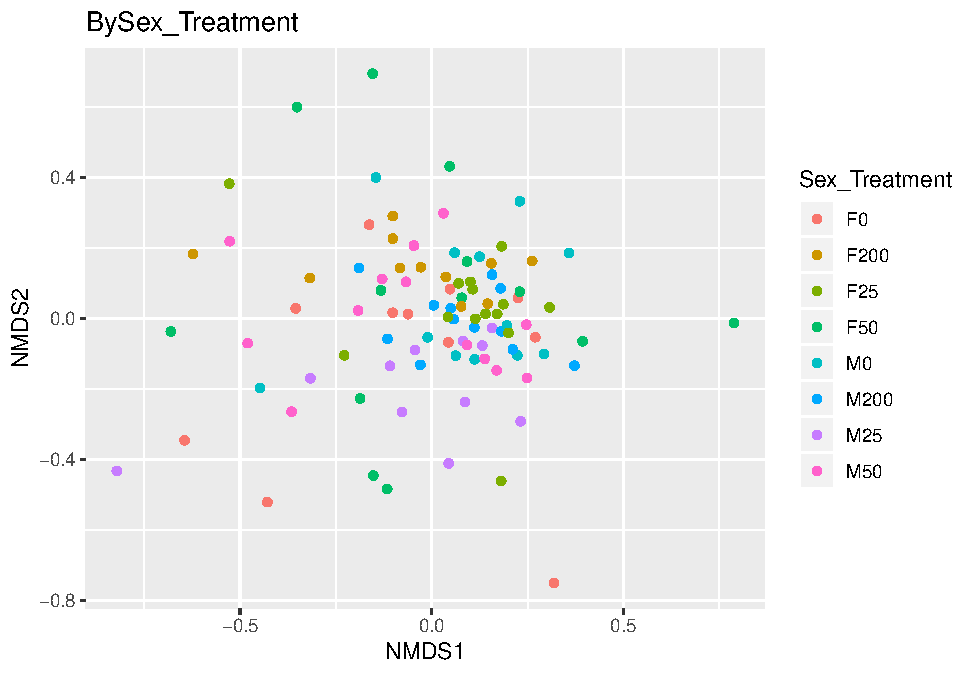
\includegraphics{Analyses_and_Plots_files/figure-latex/bray_by_Sex_Treatment-3.pdf}

\begin{verbatim}
## Square root transformation
## Wisconsin double standardization
## Run 0 stress 0.1347104 
## Run 1 stress 0.1354679 
## Run 2 stress 0.1346125 
## ... New best solution
## ... Procrustes: rmse 0.02512065  max resid 0.1530764 
## Run 3 stress 0.1359176 
## Run 4 stress 0.1348524 
## ... Procrustes: rmse 0.0298955  max resid 0.2076771 
## Run 5 stress 0.1377298 
## Run 6 stress 0.1351323 
## Run 7 stress 0.1354391 
## Run 8 stress 0.1348866 
## ... Procrustes: rmse 0.04192355  max resid 0.1678323 
## Run 9 stress 0.1343771 
## ... New best solution
## ... Procrustes: rmse 0.008675664  max resid 0.03844514 
## Run 10 stress 0.13485 
## ... Procrustes: rmse 0.03178693  max resid 0.2133193 
## Run 11 stress 0.1348765 
## ... Procrustes: rmse 0.0438577  max resid 0.2150849 
## Run 12 stress 0.1343808 
## ... Procrustes: rmse 0.01034373  max resid 0.05833612 
## Run 13 stress 0.1343881 
## ... Procrustes: rmse 0.01173177  max resid 0.05961642 
## Run 14 stress 0.1353597 
## Run 15 stress 0.1354068 
## Run 16 stress 0.1351705 
## Run 17 stress 0.1353268 
## Run 18 stress 0.1356862 
## Run 19 stress 0.1352005 
## Run 20 stress 0.1343629 
## ... New best solution
## ... Procrustes: rmse 0.005924957  max resid 0.04920202 
## Run 21 stress 0.1353091 
## Run 22 stress 0.1351894 
## Run 23 stress 0.134355 
## ... New best solution
## ... Procrustes: rmse 0.0119341  max resid 0.08455698 
## Run 24 stress 0.1343497 
## ... New best solution
## ... Procrustes: rmse 0.001673779  max resid 0.009191093 
## ... Similar to previous best
## *** Solution reached
\end{verbatim}

\includegraphics{Analyses_and_Plots_files/figure-latex/nmds_different_axes-1.pdf}
\includegraphics{Analyses_and_Plots_files/figure-latex/nmds_different_axes-2.pdf}

\begin{verbatim}
## You set `rngseed` to FALSE. Make sure you've set & recorded
##  the random seed of your session for reproducibility.
## See `?set.seed`
\end{verbatim}

\begin{verbatim}
## ...
\end{verbatim}

\begin{verbatim}
## 195OTUs were removed because they are no longer 
## present in any sample after random subsampling
\end{verbatim}

\begin{verbatim}
## ...
\end{verbatim}

\begin{verbatim}
## 
## Call:
## adonis(formula = physeq1.dist ~ Treatment * Sex, data = sampledf,      permutations = 5000) 
## 
## Permutation: free
## Number of permutations: 5000
## 
## Terms added sequentially (first to last)
## 
##               Df SumsOfSqs MeanSqs F.Model      R2 Pr(>F)    
## Treatment      1    0.2861 0.28613  1.3593 0.01386 0.0204 *  
## Sex            1    0.5376 0.53758  2.5539 0.02604 0.0002 ***
## Treatment:Sex  1    0.2414 0.24138  1.1467 0.01169 0.1512    
## Residuals     93   19.5760 0.21049         0.94840           
## Total         96   20.6411                 1.00000           
## ---
## Signif. codes:  0 '***' 0.001 '**' 0.01 '*' 0.05 '.' 0.1 ' ' 1
\end{verbatim}

\begin{verbatim}
## 
## Start: physeq1.dist ~ Treatment * Sex 
## 
##                 Df    AIC      F Pr(>F)
## - Treatment:Sex  1 294.69 1.1467  0.125
## 
## Step: physeq1.dist ~ Treatment + Sex 
## 
##                 Df   AIC      F Pr(>F)
## + Treatment:Sex  1 295.5 1.1467  0.215
## 
##             Df    AIC      F Pr(>F)   
## - Treatment  1 294.11 1.3833  0.020 * 
## - Sex        1 295.29 2.5499  0.005 **
## ---
## Signif. codes:  0 '***' 0.001 '**' 0.01 '*' 0.05 '.' 0.1 ' ' 1
## 
##                 Df   AIC      F Pr(>F)
## + Treatment:Sex  1 295.5 1.1467  0.145
\end{verbatim}

\begin{verbatim}
## Call: capscale(formula = physeq1.dist ~ Treatment + Sex, data =
## sampledf, distance = "bray")
## 
##                Inertia Proportion Rank
## Total         20.64109    1.00000     
## Constrained    0.82370    0.03991    2
## Unconstrained 19.81738    0.96009   94
## Inertia is squared Bray distance 
## 
## Eigenvalues for constrained axes:
##   CAP1   CAP2 
## 0.5743 0.2494 
## 
## Eigenvalues for unconstrained axes:
##   MDS1   MDS2   MDS3   MDS4   MDS5   MDS6   MDS7   MDS8 
## 1.4910 0.9866 0.7185 0.6243 0.5187 0.4979 0.4718 0.4628 
## (Showing 8 of 94 unconstrained eigenvalues)
\end{verbatim}

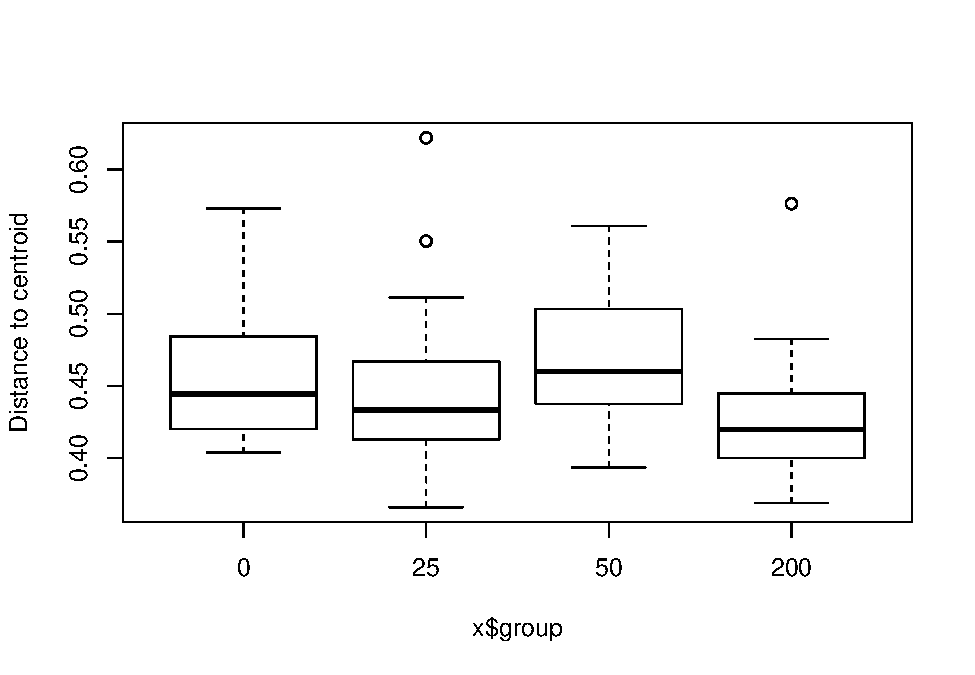
\includegraphics{Analyses_and_Plots_files/figure-latex/betadispersion-1.pdf}

\begin{verbatim}
## 
## Permutation test for homogeneity of multivariate dispersions
## Permutation: free
## Number of permutations: 5000
## 
## Response: Distances
##           Df   Sum Sq   Mean Sq      F N.Perm  Pr(>F)  
## Groups     3 0.021912 0.0073040 2.8584   5000 0.03879 *
## Residuals 93 0.237642 0.0025553                        
## ---
## Signif. codes:  0 '***' 0.001 '**' 0.01 '*' 0.05 '.' 0.1 ' ' 1
## 
## Pairwise comparisons:
## (Observed p-value below diagonal, permuted p-value above diagonal)
##             0        25        50    200
## 0             0.3829234 0.6286743 0.0320
## 25  0.3864478           0.1459708 0.1772
## 50  0.6217990 0.1438410           0.0036
## 200 0.0348478 0.1829291 0.0045218
\end{verbatim}

\begin{verbatim}
## Loading required package: S4Vectors
\end{verbatim}

\begin{verbatim}
## Loading required package: stats4
\end{verbatim}

\begin{verbatim}
## Loading required package: BiocGenerics
\end{verbatim}

\begin{verbatim}
## Loading required package: parallel
\end{verbatim}

\begin{verbatim}
## 
## Attaching package: 'BiocGenerics'
\end{verbatim}

\begin{verbatim}
## The following objects are masked from 'package:parallel':
## 
##     clusterApply, clusterApplyLB, clusterCall, clusterEvalQ,
##     clusterExport, clusterMap, parApply, parCapply, parLapply,
##     parLapplyLB, parRapply, parSapply, parSapplyLB
\end{verbatim}

\begin{verbatim}
## The following objects are masked from 'package:stats':
## 
##     IQR, mad, sd, var, xtabs
\end{verbatim}

\begin{verbatim}
## The following objects are masked from 'package:base':
## 
##     anyDuplicated, append, as.data.frame, basename, cbind,
##     colnames, dirname, do.call, duplicated, eval, evalq, Filter,
##     Find, get, grep, grepl, intersect, is.unsorted, lapply, Map,
##     mapply, match, mget, order, paste, pmax, pmax.int, pmin,
##     pmin.int, Position, rank, rbind, Reduce, rownames, sapply,
##     setdiff, sort, table, tapply, union, unique, unsplit, which,
##     which.max, which.min
\end{verbatim}

\begin{verbatim}
## 
## Attaching package: 'S4Vectors'
\end{verbatim}

\begin{verbatim}
## The following object is masked from 'package:base':
## 
##     expand.grid
\end{verbatim}

\begin{verbatim}
## Loading required package: IRanges
\end{verbatim}

\begin{verbatim}
## 
## Attaching package: 'IRanges'
\end{verbatim}

\begin{verbatim}
## The following object is masked from 'package:phyloseq':
## 
##     distance
\end{verbatim}

\begin{verbatim}
## The following object is masked from 'package:grDevices':
## 
##     windows
\end{verbatim}

\begin{verbatim}
## Loading required package: GenomicRanges
\end{verbatim}

\begin{verbatim}
## Loading required package: GenomeInfoDb
\end{verbatim}

\begin{verbatim}
## Loading required package: SummarizedExperiment
\end{verbatim}

\begin{verbatim}
## Loading required package: Biobase
\end{verbatim}

\begin{verbatim}
## Welcome to Bioconductor
## 
##     Vignettes contain introductory material; view with
##     'browseVignettes()'. To cite Bioconductor, see
##     'citation("Biobase")', and for packages 'citation("pkgname")'.
\end{verbatim}

\begin{verbatim}
## 
## Attaching package: 'Biobase'
\end{verbatim}

\begin{verbatim}
## The following object is masked from 'package:phyloseq':
## 
##     sampleNames
\end{verbatim}

\begin{verbatim}
## Loading required package: DelayedArray
\end{verbatim}

\begin{verbatim}
## Loading required package: matrixStats
\end{verbatim}

\begin{verbatim}
## 
## Attaching package: 'matrixStats'
\end{verbatim}

\begin{verbatim}
## The following objects are masked from 'package:Biobase':
## 
##     anyMissing, rowMedians
\end{verbatim}

\begin{verbatim}
## Loading required package: BiocParallel
\end{verbatim}

\begin{verbatim}
## 
## Attaching package: 'DelayedArray'
\end{verbatim}

\begin{verbatim}
## The following objects are masked from 'package:matrixStats':
## 
##     colMaxs, colMins, colRanges, rowMaxs, rowMins, rowRanges
\end{verbatim}

\begin{verbatim}
## The following objects are masked from 'package:base':
## 
##     aperm, apply, rowsum
\end{verbatim}

\begin{verbatim}
## converting counts to integer mode
\end{verbatim}

\begin{verbatim}
##   the design formula contains a numeric variable with integer values,
##   specifying a model with increasing fold change for higher values.
##   did you mean for this to be a factor? if so, first convert
##   this variable to a factor using the factor() function
\end{verbatim}

\begin{verbatim}
## estimating size factors
\end{verbatim}

\begin{verbatim}
## estimating dispersions
\end{verbatim}

\begin{verbatim}
## gene-wise dispersion estimates
\end{verbatim}

\begin{verbatim}
## mean-dispersion relationship
\end{verbatim}

\begin{verbatim}
## final dispersion estimates
\end{verbatim}

\begin{verbatim}
## fitting model and testing
\end{verbatim}

\begin{verbatim}
## -- replacing outliers and refitting for 22 genes
## -- DESeq argument 'minReplicatesForReplace' = 7 
## -- original counts are preserved in counts(dds)
\end{verbatim}

\begin{verbatim}
## estimating dispersions
\end{verbatim}

\begin{verbatim}
## fitting model and testing
\end{verbatim}

\begin{verbatim}
##        baseMean log2FoldChange       lfcSE     stat      pvalue
## ASV882 28.36935    -0.02385304 0.005376461 -4.43657 9.14038e-06
##                padj  Kingdom      Phylum      Class             Order
## ASV882 0.0008866168 Bacteria Tenericutes Mollicutes Anaeroplasmatales
##                    Family        Genus Species
## ASV882 Anaeroplasmataceae Anaeroplasma    <NA>
\end{verbatim}

\begin{verbatim}
## You set `rngseed` to FALSE. Make sure you've set & recorded
##  the random seed of your session for reproducibility.
## See `?set.seed`
\end{verbatim}

\begin{verbatim}
## ...
\end{verbatim}

\begin{verbatim}
## 195OTUs were removed because they are no longer 
## present in any sample after random subsampling
\end{verbatim}

\begin{verbatim}
## ...
\end{verbatim}

\begin{verbatim}
## You set `rngseed` to FALSE. Make sure you've set & recorded
##  the random seed of your session for reproducibility.
## See `?set.seed`
\end{verbatim}

\begin{verbatim}
## ...
\end{verbatim}

\begin{verbatim}
## 6OTUs were removed because they are no longer 
## present in any sample after random subsampling
\end{verbatim}

\begin{verbatim}
## ...
\end{verbatim}

\begin{verbatim}
## converting counts to integer mode
\end{verbatim}

\begin{verbatim}
## estimating size factors
\end{verbatim}

\begin{verbatim}
## estimating dispersions
\end{verbatim}

\begin{verbatim}
## gene-wise dispersion estimates
\end{verbatim}

\begin{verbatim}
## mean-dispersion relationship
\end{verbatim}

\begin{verbatim}
## final dispersion estimates
\end{verbatim}

\begin{verbatim}
## fitting model and testing
\end{verbatim}

\begin{verbatim}
## [1] "No significant taxa were identified using the specified formula"
\end{verbatim}

\begin{verbatim}
## converting counts to integer mode
\end{verbatim}

\begin{verbatim}
## estimating size factors
\end{verbatim}

\begin{verbatim}
## estimating dispersions
\end{verbatim}

\begin{verbatim}
## gene-wise dispersion estimates
\end{verbatim}

\begin{verbatim}
## mean-dispersion relationship
\end{verbatim}

\begin{verbatim}
## final dispersion estimates
\end{verbatim}

\begin{verbatim}
## fitting model and testing
\end{verbatim}

\begin{verbatim}
## [1] "No significant taxa were identified using the specified formula"
\end{verbatim}

\begin{verbatim}
## converting counts to integer mode
\end{verbatim}

\begin{verbatim}
## estimating size factors
\end{verbatim}

\begin{verbatim}
## estimating dispersions
\end{verbatim}

\begin{verbatim}
## gene-wise dispersion estimates
\end{verbatim}

\begin{verbatim}
## mean-dispersion relationship
\end{verbatim}

\begin{verbatim}
## final dispersion estimates
\end{verbatim}

\begin{verbatim}
## fitting model and testing
\end{verbatim}

\begin{verbatim}
## 1 rows did not converge in beta, labelled in mcols(object)$betaConv. Use larger maxit argument with nbinomWaldTest
\end{verbatim}

\begin{verbatim}
## -- replacing outliers and refitting for 3841 genes
## -- DESeq argument 'minReplicatesForReplace' = 7 
## -- original counts are preserved in counts(dds)
\end{verbatim}

\begin{verbatim}
## estimating dispersions
\end{verbatim}

\begin{verbatim}
## fitting model and testing
\end{verbatim}

\begin{verbatim}
##          baseMean log2FoldChange      lfcSE       stat        pvalue
## ASV1274 2.8320397      0.4321006 0.07989097   5.408629  6.350899e-08
## ASV1962 1.1447545     -1.9638202 0.07989418 -24.580265 2.053843e-133
## ASV1972 1.1367492     -1.9624451 0.07989418 -24.563054 3.137200e-133
## ASV2074 1.8190865     -7.7935595 0.07994057 -97.491923  0.000000e+00
## ASV2252 0.8885856     -1.9144467 0.07989430 -23.962243 6.887826e-127
## ASV2257 1.5532200     -7.7235466 0.07994060 -96.616067  0.000000e+00
## ASV2295 0.2378805     -6.9423604 0.07994198 -86.842487  0.000000e+00
## ASV2307 1.4972481     -7.7080044 0.07994061 -96.421634  0.000000e+00
## ASV2327 1.4552692     -7.6958199 0.07994062 -96.269206  0.000000e+00
## ASV2583 0.6724432     -1.8602894 0.07989448 -23.284330 6.390388e-120
## ASV2657 0.6324168     -1.8483406 0.07989452 -23.134759 2.069914e-118
## ASV2659 1.1054449     -7.5983535 0.07994070 -95.049870  0.000000e+00
## ASV2741 0.5923904     -1.8355209 0.07989458 -22.974286 8.427416e-117
## ASV2776 0.5763799     -1.8302231 0.07989460 -22.907971 3.869544e-116
## ASV2843 0.9515222     -7.5371599 0.07994076 -94.284316  0.000000e+00
## ASV2910 0.5123377     -1.8077804 0.07989470 -22.627037 2.348616e-113
## ASV3092 0.4322849     -1.7746987 0.07989488 -22.212921 2.576331e-109
## ASV3255 0.6436768     -7.3877184 0.07994095 -92.414689  0.000000e+00
## ASV3271 0.3602374     -1.7397148 0.07989511 -21.774985 4.005977e-105
## ASV3317 0.6016978     -7.3031903 0.07994100 -91.357258  0.000000e+00
## ASV3434 0.3042005     -1.7068887 0.07989536 -21.364053 2.886449e-101
## ASV3435 0.3042005     -1.7068887 0.07989536 -21.364053 2.886449e-101
## ASV3710 0.2321530     -1.6548384 0.07989587 -20.712441  2.675495e-95
## ASV3746 0.2241477     -1.6481255 0.07989594 -20.628401  1.526146e-94
## ASV3799 0.2161425     -1.6411483 0.07989602 -20.541051  9.253836e-94
## ASV3806 0.3778103     -7.1363186 0.07994138 -89.269397  0.000000e+00
## ASV3846 0.3638173     -7.1530217 0.07994142 -89.478295  0.000000e+00
## ASV3891 0.3498243     -7.2869158 0.07994146 -91.153149  0.000000e+00
## ASV3985 0.3078454     -7.0697225 0.07994161 -88.436078  0.000000e+00
## ASV4084 0.2798595     -7.0054031 0.07994174 -87.631360  0.000000e+00
## ASV4474 0.1819086     -6.8533338 0.07994248 -85.728310  0.000000e+00
## ASV4475 0.1819086     -6.8533338 0.07994248 -85.728310  0.000000e+00
##                  padj  Kingdom        Phylum       Class           Order
## ASV1274  6.025415e-06 Bacteria Bacteroidetes Bacteroidia   Bacteroidales
## ASV1962 3.667922e-131 Bacteria    Firmicutes  Clostridia   Clostridiales
## ASV1972 5.291411e-131 Bacteria    Firmicutes  Clostridia   Clostridiales
## ASV2074  0.000000e+00 Bacteria    Firmicutes  Clostridia   Clostridiales
## ASV2252 1.100602e-124 Bacteria    Firmicutes  Clostridia   Clostridiales
## ASV2257  0.000000e+00 Bacteria Bacteroidetes Bacteroidia   Bacteroidales
## ASV2295  0.000000e+00 Bacteria   Tenericutes  Mollicutes Mollicutes_RF39
## ASV2307  0.000000e+00 Bacteria Bacteroidetes Bacteroidia   Bacteroidales
## ASV2327  0.000000e+00 Bacteria    Firmicutes  Clostridia   Clostridiales
## ASV2583 9.700609e-118 Bacteria    Firmicutes  Clostridia   Clostridiales
## ASV2657 2.992504e-116 Bacteria    Firmicutes  Clostridia   Clostridiales
## ASV2659  0.000000e+00 Bacteria    Firmicutes  Clostridia   Clostridiales
## ASV2741 1.162983e-114 Bacteria    Firmicutes  Clostridia   Clostridiales
## ASV2776 5.107797e-114 Bacteria Bacteroidetes Bacteroidia   Bacteroidales
## ASV2843  0.000000e+00 Bacteria Bacteroidetes Bacteroidia   Bacteroidales
## ASV2910 2.970999e-111 Bacteria    Firmicutes  Clostridia   Clostridiales
## ASV3092 3.128697e-107 Bacteria    Firmicutes  Clostridia   Clostridiales
## ASV3255  0.000000e+00 Bacteria    Firmicutes  Clostridia   Clostridiales
## ASV3271 4.677748e-103 Bacteria    Firmicutes  Clostridia   Clostridiales
## ASV3317  0.000000e+00 Bacteria    Firmicutes  Clostridia   Clostridiales
## ASV3434  3.129736e-99 Bacteria    Firmicutes  Clostridia   Clostridiales
## ASV3435  3.129736e-99 Bacteria    Firmicutes  Clostridia   Clostridiales
## ASV3710  2.800967e-93 Bacteria    Firmicutes  Clostridia   Clostridiales
## ASV3746  1.544459e-92 Bacteria    Firmicutes  Clostridia   Clostridiales
## ASV3799  9.062789e-92 Bacteria Bacteroidetes Bacteroidia   Bacteroidales
## ASV3806  0.000000e+00 Bacteria    Firmicutes  Clostridia   Clostridiales
## ASV3846  0.000000e+00 Bacteria    Firmicutes  Clostridia   Clostridiales
## ASV3891  0.000000e+00 Bacteria    Firmicutes  Clostridia   Clostridiales
## ASV3985  0.000000e+00 Bacteria Bacteroidetes Bacteroidia   Bacteroidales
## ASV4084  0.000000e+00 Bacteria Bacteroidetes Bacteroidia   Bacteroidales
## ASV4474  0.000000e+00 Bacteria    Firmicutes  Clostridia   Clostridiales
## ASV4475  0.000000e+00 Bacteria Bacteroidetes Bacteroidia   Bacteroidales
##                  Family                        Genus Species
## ASV1274  Muribaculaceae                         <NA>    <NA>
## ASV1962 Lachnospiraceae                         <NA>    <NA>
## ASV1972 Lachnospiraceae                         <NA>    <NA>
## ASV2074 Ruminococcaceae          Ruminiclostridium_9    <NA>
## ASV2252 Lachnospiraceae                         <NA>    <NA>
## ASV2257  Muribaculaceae                         <NA>    <NA>
## ASV2295            <NA>                         <NA>    <NA>
## ASV2307  Muribaculaceae                  Muribaculum    <NA>
## ASV2327 Lachnospiraceae                         <NA>    <NA>
## ASV2583 Lachnospiraceae                         <NA>    <NA>
## ASV2657 Lachnospiraceae                         <NA>    <NA>
## ASV2659 Lachnospiraceae                         <NA>    <NA>
## ASV2741 Lachnospiraceae                         <NA>    <NA>
## ASV2776  Muribaculaceae                         <NA>    <NA>
## ASV2843  Muribaculaceae                         <NA>    <NA>
## ASV2910 Lachnospiraceae                    UC5-1-2E3    <NA>
## ASV3092 Lachnospiraceae                Acetatifactor    <NA>
## ASV3255 Ruminococcaceae            Ruminiclostridium    <NA>
## ASV3271 Lachnospiraceae                         <NA>    <NA>
## ASV3317 Lachnospiraceae                           A2    <NA>
## ASV3434 Lachnospiraceae                         <NA>    <NA>
## ASV3435 Lachnospiraceae Lachnospiraceae_FCS020_group    <NA>
## ASV3710 Ruminococcaceae               Butyricicoccus    <NA>
## ASV3746 Lachnospiraceae                 Tyzzerella_3    <NA>
## ASV3799   Rikenellaceae                    Alistipes    <NA>
## ASV3806 Lachnospiraceae                GCA-900066575    <NA>
## ASV3846 Lachnospiraceae                       ASF356    <NA>
## ASV3891 Ruminococcaceae            Ruminiclostridium    <NA>
## ASV3985  Muribaculaceae                      CAG-873    <NA>
## ASV4084   Rikenellaceae                    Alistipes    <NA>
## ASV4474 Lachnospiraceae                 Tyzzerella_3    <NA>
## ASV4475  Muribaculaceae                         <NA>    <NA>
\end{verbatim}

\begin{verbatim}
## converting counts to integer mode
\end{verbatim}

\begin{verbatim}
## estimating size factors
\end{verbatim}

\begin{verbatim}
## estimating dispersions
\end{verbatim}

\begin{verbatim}
## gene-wise dispersion estimates
\end{verbatim}

\begin{verbatim}
## mean-dispersion relationship
\end{verbatim}

\begin{verbatim}
## final dispersion estimates
\end{verbatim}

\begin{verbatim}
## fitting model and testing
\end{verbatim}

\begin{verbatim}
## -- replacing outliers and refitting for 22 genes
## -- DESeq argument 'minReplicatesForReplace' = 7 
## -- original counts are preserved in counts(dds)
\end{verbatim}

\begin{verbatim}
## estimating dispersions
\end{verbatim}

\begin{verbatim}
## fitting model and testing
\end{verbatim}

\begin{verbatim}
## [1] "No significant taxa were identified using the specified formula"
\end{verbatim}

\begin{verbatim}
## converting counts to integer mode
\end{verbatim}

\begin{verbatim}
## estimating size factors
\end{verbatim}

\begin{verbatim}
## estimating dispersions
\end{verbatim}

\begin{verbatim}
## gene-wise dispersion estimates
\end{verbatim}

\begin{verbatim}
## mean-dispersion relationship
\end{verbatim}

\begin{verbatim}
## final dispersion estimates
\end{verbatim}

\begin{verbatim}
## fitting model and testing
\end{verbatim}

\begin{verbatim}
## 2 rows did not converge in beta, labelled in mcols(object)$betaConv. Use larger maxit argument with nbinomWaldTest
\end{verbatim}

\begin{verbatim}
##           baseMean log2FoldChange      lfcSE        stat       pvalue
## ASV606  8.40571923      0.7619289 0.09296904    8.195512 2.495282e-16
## ASV1483 3.29221595      0.4011197 0.09328930    4.299739 1.709993e-05
## ASV1702 2.61355740      0.3975148 0.09330048    4.260587 2.038911e-05
## ASV1727 2.54135968      0.3970808 0.09330197    4.255868 2.082400e-05
## ASV1870 1.69475384     -0.9796158 0.09329203  -10.500530 8.589631e-26
## ASV1871 1.69475384     -0.9796158 0.09329203  -10.500530 8.589631e-26
## ASV1881 1.35544876     -0.9230846 0.09326713   -9.897212 4.280427e-23
## ASV1909 1.56362909     -1.1561008 0.09339715  -12.378331 3.423901e-35
## ASV1923 1.15724495     -1.3781911 0.09345399  -14.747269 3.203700e-49
## ASV1961 1.25944355     -0.9453099 0.09327787  -10.134343 3.889799e-24
## ASV1993 1.45868754     -1.1598950 0.09340183  -12.418333 2.078479e-35
## ASV2077 1.46978134      0.3604334 0.09344422    3.857204 1.146916e-04
## ASV2097 1.55397008      0.3656383 0.09342126    3.913866 9.083010e-05
## ASV2104 1.32226353     -1.1652481 0.09340588  -12.475105 1.020716e-35
## ASV2168 1.24880444     -1.1683564 0.09340593  -12.508375 6.718490e-36
## ASV2373 1.42499849     -0.9925814 0.09329793  -10.638836 1.965688e-26
## ASV2420 1.36856291     -0.9942511 0.09329880  -10.656633 1.623701e-26
## ASV2470 0.97595641     -1.1816976 0.09340621  -12.651167 1.102246e-36
## ASV2488 0.72426214     -1.3661746 0.09345426  -14.618644 2.136118e-48
## ASV2539 0.90362935      0.3554094 0.09345843    3.802861 1.430346e-04
## ASV2565 0.89200317     -1.1865353 0.09340633  -12.702943 5.694708e-37
## ASV2579 0.88150902     -1.1862044 0.09340634  -12.699399 5.958565e-37
## ASV2606 1.00335076      0.3596393 0.09344668    3.848604 1.187927e-04
## ASV2609 0.86052071     -1.1824502 0.09340638  -12.659201 9.950728e-37
## ASV2627 0.85002655     -1.1805311 0.09340640  -12.638653 1.292497e-36
## ASV2665 0.95440682      0.3589534 0.09344889    3.841173 1.224478e-04
## ASV2725 0.59043110     -1.3522065 0.09345442  -14.469154 1.897912e-47
## ASV2734 0.76860428      0.3532383 0.09346379    3.779413 1.571986e-04
## ASV2770 0.74783119      0.3528716 0.09346477    3.775450 1.597191e-04
## ASV2772 0.75557916     -1.1622725 0.09340662  -12.443150 1.523746e-35
## ASV2786 0.73744464      0.3526799 0.09346529    3.773379 1.610515e-04
## ASV2789 0.74508500     -1.1600815 0.09340664  -12.419689 2.043537e-35
## ASV2836 0.71360254     -1.1533382 0.09340673  -12.347485 5.025825e-35
## ASV2849 0.69589847      0.3519073 0.09346744    3.765026 1.665318e-04
## ASV2854 0.70310838     -1.1510395 0.09340676  -12.322871 6.822118e-35
## ASV3019 0.45660005     -1.3437578 0.09345468  -14.378710 7.039426e-47
## ASV3020 0.45660005     -1.3437578 0.09345468  -14.378710 7.039426e-47
## ASV3073 0.57717852     -1.1204921 0.09340721  -11.995778 3.738867e-33
## ASV3141 0.40936556    -29.9932081 0.09345482 -320.938069 0.000000e+00
## ASV3215 0.37787590    -29.9931705 0.09345492 -320.937298 0.000000e+00
## ASV3334 0.33064141     -1.3012239 0.09345512  -13.923516 4.559097e-44
## ASV3400 0.40927204     -1.0676351 0.09340822  -11.429776 2.968728e-30
## ASV3436 0.29915175     -1.2902442 0.09345529  -13.806005 2.344789e-43
## ASV3524 0.27553451     -1.3215589 0.09345544  -14.141059 2.120674e-45
## ASV3525 0.27553451     -1.3215589 0.09345544  -14.141059 2.120674e-45
## ASV3606 0.25191727     -1.2819988 0.09345562  -13.717729 7.951735e-43
## ASV3648 0.24404485     -1.2826722 0.09345568  -13.724925 7.200377e-43
## ASV3749 0.22042761     -1.2743940 0.09345591  -13.636312 2.435722e-42
## ASV3750 0.22042761     -1.2743940 0.09345591  -13.636312 2.435722e-42
## ASV3803 0.21255519     -1.2807307 0.09345600  -13.704103 9.594580e-43
## ASV4064 0.20988310     -0.9665879 0.09341152  -10.347631 4.289709e-25
## ASV4278 0.16790648     -0.9333116 0.09341320   -9.991217 1.665239e-23
## ASV4279 0.16790648     -0.9333116 0.09341320   -9.991217 1.665239e-23
## ASV4280 0.16790648     -0.9333116 0.09341320   -9.991217 1.665239e-23
## ASV5057 0.04723449     -1.1805183 0.09346463  -12.630643 1.431044e-36
## ASV5058 0.04723449     -1.1805183 0.09346463  -12.630643 1.431044e-36
## ASV5184 0.03936207     -1.1594156 0.09346688  -12.404560 2.468640e-35
##                 padj  Kingdom         Phylum               Class
## ASV606  3.216696e-14 Bacteria     Firmicutes          Clostridia
## ASV1483 2.156450e-03 Bacteria  Bacteroidetes         Bacteroidia
## ASV1702 2.516536e-03 Bacteria  Bacteroidetes         Bacteroidia
## ASV1727 2.516667e-03 Bacteria  Bacteroidetes         Bacteroidia
## ASV1870 1.311275e-23 Bacteria  Bacteroidetes         Bacteroidia
## ASV1871 1.311275e-23 Bacteria     Firmicutes          Clostridia
## ASV1881 5.643354e-21 Bacteria     Firmicutes          Clostridia
## ASV1909 6.620683e-33 Bacteria  Bacteroidetes         Bacteroidia
## ASV1923 6.194888e-46 Bacteria     Firmicutes          Clostridia
## ASV1961 5.641182e-22 Bacteria  Bacteroidetes         Bacteroidia
## ASV1993 4.306163e-33 Bacteria     Firmicutes          Clostridia
## ASV2077 1.330652e-02 Bacteria     Firmicutes          Clostridia
## ASV2097 1.075317e-02 Bacteria  Bacteroidetes         Bacteroidia
## ASV2104 2.368469e-33 Bacteria     Firmicutes          Clostridia
## ASV2168 1.623915e-33 Bacteria     Firmicutes          Clostridia
## ASV2373 3.167488e-24 Bacteria     Firmicutes          Clostridia
## ASV2420 2.691168e-24 Bacteria     Firmicutes          Clostridia
## ASV2470 3.197066e-34 Bacteria  Bacteroidetes         Bacteroidia
## ASV2488 3.097906e-45 Bacteria     Firmicutes          Clostridia
## ASV2539 1.565554e-02 Bacteria     Firmicutes          Clostridia
## ASV2565 1.920313e-34 Bacteria     Firmicutes          Clostridia
## ASV2579 1.920313e-34 Bacteria     Firmicutes          Clostridia
## ASV2606 1.351209e-02 Bacteria     Firmicutes          Clostridia
## ASV2609 3.038114e-34 Bacteria     Firmicutes          Clostridia
## ASV2627 3.570368e-34 Bacteria     Firmicutes          Clostridia
## ASV2665 1.365999e-02 Bacteria     Firmicutes          Clostridia
## ASV2725 2.201958e-44 Bacteria     Firmicutes          Clostridia
## ASV2734 1.668321e-02 Bacteria     Firmicutes          Clostridia
## ASV2770 1.668321e-02 Bacteria  Bacteroidetes         Bacteroidia
## ASV2772 3.399711e-33 Bacteria     Firmicutes          Clostridia
## ASV2786 1.668321e-02 Bacteria     Firmicutes          Clostridia
## ASV2789 4.306163e-33 Bacteria     Firmicutes          Clostridia
## ASV2836 9.404778e-33 Bacteria     Firmicutes          Clostridia
## ASV2849 1.694826e-02 Bacteria     Firmicutes          Clostridia
## ASV2854 1.236722e-32 Bacteria     Firmicutes          Clostridia
## ASV3019 5.833673e-44 Bacteria Proteobacteria Deltaproteobacteria
## ASV3020 5.833673e-44 Bacteria  Bacteroidetes         Bacteroidia
## ASV3073 6.572475e-31 Bacteria     Firmicutes          Clostridia
## ASV3141 0.000000e+00 Bacteria     Firmicutes          Clostridia
## ASV3215 0.000000e+00 Bacteria     Firmicutes          Clostridia
## ASV3334 2.644732e-41 Bacteria     Firmicutes          Clostridia
## ASV3400 5.065174e-28 Bacteria           <NA>                <NA>
## ASV3436 1.236556e-40 Bacteria     Firmicutes          Clostridia
## ASV3524 1.366892e-42 Bacteria     Firmicutes    Erysipelotrichia
## ASV3525 1.366892e-42 Bacteria     Firmicutes          Clostridia
## ASV3606 3.548309e-40 Bacteria     Firmicutes          Clostridia
## ASV3648 3.480782e-40 Bacteria     Firmicutes                <NA>
## ASV3749 8.831015e-40 Bacteria    Tenericutes          Mollicutes
## ASV3750 8.831015e-40 Bacteria     Firmicutes    Erysipelotrichia
## ASV3803 3.975583e-40 Bacteria  Bacteroidetes         Bacteroidia
## ASV4064 6.380668e-23 Bacteria     Firmicutes          Clostridia
## ASV4278 2.246524e-21 Bacteria     Firmicutes          Clostridia
## ASV4279 2.246524e-21 Bacteria  Bacteroidetes         Bacteroidia
## ASV4280 2.246524e-21 Bacteria     Firmicutes          Clostridia
## ASV5057 3.609341e-34 Bacteria    Tenericutes          Mollicutes
## ASV5058 3.609341e-34 Bacteria     Firmicutes          Clostridia
## ASV5184 4.938130e-33 Bacteria Proteobacteria Deltaproteobacteria
##                      Order                        Family
## ASV606       Clostridiales               Lachnospiraceae
## ASV1483      Bacteroidales                Muribaculaceae
## ASV1702      Bacteroidales                Bacteroidaceae
## ASV1727      Bacteroidales                Muribaculaceae
## ASV1870      Bacteroidales                Prevotellaceae
## ASV1871      Clostridiales               Lachnospiraceae
## ASV1881      Clostridiales               Lachnospiraceae
## ASV1909      Bacteroidales                Muribaculaceae
## ASV1923      Clostridiales               Lachnospiraceae
## ASV1961      Bacteroidales                Muribaculaceae
## ASV1993      Clostridiales               Ruminococcaceae
## ASV2077      Clostridiales               Ruminococcaceae
## ASV2097      Bacteroidales                Muribaculaceae
## ASV2104      Clostridiales               Lachnospiraceae
## ASV2168      Clostridiales               Ruminococcaceae
## ASV2373      Clostridiales               Lachnospiraceae
## ASV2420      Clostridiales               Lachnospiraceae
## ASV2470      Bacteroidales                Muribaculaceae
## ASV2488      Clostridiales               Ruminococcaceae
## ASV2539      Clostridiales               Lachnospiraceae
## ASV2565      Clostridiales               Lachnospiraceae
## ASV2579      Clostridiales               Lachnospiraceae
## ASV2606      Clostridiales               Lachnospiraceae
## ASV2609      Clostridiales               Lachnospiraceae
## ASV2627      Clostridiales               Ruminococcaceae
## ASV2665      Clostridiales               Lachnospiraceae
## ASV2725      Clostridiales               Lachnospiraceae
## ASV2734      Clostridiales               Lachnospiraceae
## ASV2770      Bacteroidales                Prevotellaceae
## ASV2772      Clostridiales               Ruminococcaceae
## ASV2786      Clostridiales               Ruminococcaceae
## ASV2789      Clostridiales               Ruminococcaceae
## ASV2836      Clostridiales               Lachnospiraceae
## ASV2849      Clostridiales               Lachnospiraceae
## ASV2854      Clostridiales               Ruminococcaceae
## ASV3019 Desulfovibrionales           Desulfovibrionaceae
## ASV3020      Bacteroidales                Muribaculaceae
## ASV3073      Clostridiales               Lachnospiraceae
## ASV3141      Clostridiales               Lachnospiraceae
## ASV3215      Clostridiales               Lachnospiraceae
## ASV3334      Clostridiales               Lachnospiraceae
## ASV3400               <NA>                          <NA>
## ASV3436      Clostridiales Clostridiales_vadinBB60_group
## ASV3524 Erysipelotrichales           Erysipelotrichaceae
## ASV3525      Clostridiales               Lachnospiraceae
## ASV3606      Clostridiales               Lachnospiraceae
## ASV3648               <NA>                          <NA>
## ASV3749    Mollicutes_RF39                          <NA>
## ASV3750 Erysipelotrichales           Erysipelotrichaceae
## ASV3803      Bacteroidales                Muribaculaceae
## ASV4064      Clostridiales               Lachnospiraceae
## ASV4278      Clostridiales               Ruminococcaceae
## ASV4279      Bacteroidales                          <NA>
## ASV4280      Clostridiales                          <NA>
## ASV5057    Mycoplasmatales              Mycoplasmataceae
## ASV5058      Clostridiales               Lachnospiraceae
## ASV5184 Desulfovibrionales           Desulfovibrionaceae
##                                 Genus Species
## ASV606  Lachnospiraceae_NK4A136_group    <NA>
## ASV1483                          <NA>    <NA>
## ASV1702                   Bacteroides    <NA>
## ASV1727                          <NA>    <NA>
## ASV1870        Prevotellaceae_UCG-001    <NA>
## ASV1871 Lachnospiraceae_NK4A136_group    <NA>
## ASV1881                          <NA>    <NA>
## ASV1909                          <NA>    <NA>
## ASV1923                          <NA>    <NA>
## ASV1961                          <NA>    <NA>
## ASV1993                 Oscillibacter    <NA>
## ASV2077       Ruminococcaceae_UCG-014    <NA>
## ASV2097                          <NA>    <NA>
## ASV2104 Lachnospiraceae_NK4A136_group    <NA>
## ASV2168       Ruminococcaceae_UCG-014    <NA>
## ASV2373 Lachnospiraceae_NK4A136_group    <NA>
## ASV2420                            A2    <NA>
## ASV2470                          <NA>    <NA>
## ASV2488          Pseudoflavonifractor    <NA>
## ASV2539 Lachnospiraceae_NK4A136_group    <NA>
## ASV2565                          <NA>    <NA>
## ASV2579                          <NA>    <NA>
## ASV2606 Lachnospiraceae_NK4A136_group    <NA>
## ASV2609                 GCA-900066575    <NA>
## ASV2627          Pseudoflavonifractor    <NA>
## ASV2665       Lachnospiraceae_UCG-001    <NA>
## ASV2725                     UC5-1-2E3    <NA>
## ASV2734             Lachnoclostridium    <NA>
## ASV2770        Prevotellaceae_UCG-001    <NA>
## ASV2772       Ruminococcaceae_UCG-014    <NA>
## ASV2786       Ruminococcaceae_UCG-014    <NA>
## ASV2789       Ruminococcaceae_UCG-014    <NA>
## ASV2836                          <NA>    <NA>
## ASV2849                     Roseburia    <NA>
## ASV2854           Ruminiclostridium_5    <NA>
## ASV3019                 Desulfovibrio    <NA>
## ASV3020                          <NA>    <NA>
## ASV3073                     UC5-1-2E3    <NA>
## ASV3141                          <NA>    <NA>
## ASV3215                          <NA>    <NA>
## ASV3334       Lachnospiraceae_UCG-006    <NA>
## ASV3400                          <NA>    <NA>
## ASV3436                          <NA>    <NA>
## ASV3524        Erysipelatoclostridium    <NA>
## ASV3525                 Acetatifactor    <NA>
## ASV3606                          <NA>    <NA>
## ASV3648                          <NA>    <NA>
## ASV3749                          <NA>    <NA>
## ASV3750       Candidatus_Stoquefichus    <NA>
## ASV3803                       CAG-873    <NA>
## ASV4064                 GCA-900066575    <NA>
## ASV4278                          <NA>    <NA>
## ASV4279                          <NA>    <NA>
## ASV4280                          <NA>    <NA>
## ASV5057                    Mycoplasma    <NA>
## ASV5058                          <NA>    <NA>
## ASV5184                 Desulfovibrio    <NA>
\end{verbatim}

\begin{verbatim}
## converting counts to integer mode
\end{verbatim}

\begin{verbatim}
## estimating size factors
\end{verbatim}

\begin{verbatim}
## estimating dispersions
\end{verbatim}

\begin{verbatim}
## gene-wise dispersion estimates
\end{verbatim}

\begin{verbatim}
## mean-dispersion relationship
\end{verbatim}

\begin{verbatim}
## final dispersion estimates
\end{verbatim}

\begin{verbatim}
## fitting model and testing
\end{verbatim}

\begin{verbatim}
##         baseMean log2FoldChange      lfcSE      stat       pvalue
## ASV1131 15.42357     -0.1165207 0.02956987 -3.940521 8.130496e-05
##                padj  Kingdom     Phylum      Class         Order
## ASV1131 0.008293106 Bacteria Firmicutes Clostridia Clostridiales
##                  Family  Genus Species
## ASV1131 Ruminococcaceae Phocea    <NA>
\end{verbatim}

\begin{verbatim}
## converting counts to integer mode
\end{verbatim}

\begin{verbatim}
## estimating size factors
\end{verbatim}

\begin{verbatim}
## estimating dispersions
\end{verbatim}

\begin{verbatim}
## gene-wise dispersion estimates
\end{verbatim}

\begin{verbatim}
## mean-dispersion relationship
\end{verbatim}

\begin{verbatim}
## final dispersion estimates
\end{verbatim}

\begin{verbatim}
## fitting model and testing
\end{verbatim}

\begin{verbatim}
##           baseMean log2FoldChange     lfcSE      stat       pvalue
## ASV767  7.34537648     -1.6476179 0.2138736 -7.703700 1.321815e-14
## ASV1432 2.46793653      1.2884134 0.2138174  6.025764 1.683122e-09
## ASV1456 2.25066357      0.9351587 0.2141072  4.367713 1.255544e-05
## ASV1685 1.76222169      0.9272422 0.2141077  4.330728 1.486171e-05
## ASV1723 1.69518065      0.9259898 0.2141078  4.324877 1.526168e-05
## ASV1747 1.77158929      1.2724894 0.2138350  5.950801 2.668337e-09
## ASV1804 1.56109856      0.9233282 0.2141080  4.312442 1.614613e-05
## ASV1924 1.49509848      1.2643522 0.2138397  5.912617 3.367150e-09
## ASV1935 1.48485808      1.2640254 0.2138399  5.911083 3.398657e-09
## ASV1989 1.33124356      0.9181820 0.2141084  4.288398 1.799663e-05
## ASV2007 1.31208898      0.9177182 0.2141084  4.286231 1.817299e-05
## ASV2042 1.27377981      0.9167622 0.2141085  4.281764 1.854175e-05
## ASV2164 1.22884806      1.2549678 0.2138460  5.868558 4.396022e-09
## ASV2172 1.14537193      1.1764005 0.2139576  5.498287 3.834985e-08
## ASV2285 1.03434751      0.9100482 0.2141092  4.250393 2.133955e-05
## ASV2348 1.04452085      1.2471984 0.2138521  5.832060 5.474726e-09
## ASV2519 0.90115525      1.2401485 0.2138584  5.798923 6.674201e-09
## ASV2711 0.76803004      1.2325243 0.2138661  5.763065 8.260017e-09
## ASV2732 0.75778964      1.2318845 0.2138668  5.760054 8.408698e-09
## ASV2815 0.66083313      0.8956231 0.2141111  4.182982 2.877098e-05
## ASV2880 0.62252397      0.8937022 0.2141114  4.174005 2.992918e-05
## ASV2896 0.61294667      0.8932042 0.2141115  4.171677 3.023660e-05
## ASV2945 0.62514690      1.3140919 0.2136449  6.150821 7.708271e-10
## ASV3025 0.54590563      0.8894782 0.2141122  4.154262 3.263391e-05
## ASV3063 0.52675105      0.8883254 0.2141124  4.148873 3.341159e-05
## ASV3181 0.46928730      0.8846146 0.2141132  4.131527 3.603611e-05
## ASV3392 0.37351438      0.8772797 0.2141150  4.097236 4.181124e-05
## ASV3403 0.48609437      0.7026890 0.2131761  3.296284 9.797289e-04
## ASV3418 0.36393709      0.8764398 0.2141152  4.093309 4.252604e-05
## ASV3419 0.36393709      0.8764398 0.2141152  4.093309 4.252604e-05
## ASV3619 0.29689605      0.8698906 0.2141172  4.062685 4.851157e-05
## ASV3660 0.28731875      0.8688339 0.2141175  4.057743 4.954934e-05
## ASV3722 0.26816417      0.8666181 0.2141183  4.047379 5.179423e-05
## ASV3816 0.24900959      0.8642304 0.2141192  4.036212 5.432125e-05
## ASV3854 0.23943229      0.8629694 0.2141197  4.030313 5.570258e-05
## ASV3895 0.22985500      0.8616543 0.2141202  4.024161 5.717867e-05
## ASV4037 0.19154584      0.8557781 0.2141228  3.996669 6.424005e-05
## ASV4149 0.17239125      0.8523798 0.2141245  3.980766 6.869345e-05
## ASV4200 0.16281396      0.8505316 0.2141255  3.972117 7.123683e-05
## ASV4257 0.15323667      0.8473095 0.2141231  3.957113 7.586090e-05
## ASV4380 0.13408209      0.8442510 0.2141293  3.942715 8.056431e-05
## ASV4381 0.13408209      0.8442510 0.2141293  3.942715 8.056431e-05
## ASV4434 0.12450479      0.8418520 0.2141310  3.931481 8.442403e-05
## ASV4872 0.06704104      0.8216857 0.2141499  3.836966 1.245637e-04
## ASV4981 0.05746375      0.8166277 0.2141565  3.813230 1.371626e-04
## ASV4982 0.05746375      0.8166277 0.2141565  3.813230 1.371626e-04
## ASV4983 0.05746375      0.8166277 0.2141565  3.813230 1.371626e-04
## ASV4984 0.05746375      0.8166277 0.2141565  3.813230 1.371626e-04
## ASV5104 0.04788646      0.8106212 0.2141656  3.785021 1.536954e-04
## ASV5232 0.03830917      0.8032299 0.2141790  3.750274 1.766416e-04
## ASV5233 0.03830917      0.8032299 0.2141790  3.750274 1.766416e-04
##                 padj  Kingdom        Phylum       Class           Order
## ASV767  6.726716e-11 Bacteria Bacteroidetes Bacteroidia   Bacteroidales
## ASV1432 2.855137e-06 Bacteria Bacteroidetes Bacteroidia   Bacteroidales
## ASV1456 4.914973e-03 Bacteria Bacteroidetes Bacteroidia   Bacteroidales
## ASV1685 4.966261e-03 Bacteria Bacteroidetes Bacteroidia   Bacteroidales
## ASV1723 4.966261e-03 Bacteria Bacteroidetes Bacteroidia   Bacteroidales
## ASV1747 2.882628e-06 Bacteria Bacteroidetes Bacteroidia   Bacteroidales
## ASV1804 4.966261e-03 Bacteria    Firmicutes  Clostridia   Clostridiales
## ASV1924 2.882628e-06 Bacteria Bacteroidetes Bacteroidia   Bacteroidales
## ASV1935 2.882628e-06 Bacteria Bacteroidetes Bacteroidia   Bacteroidales
## ASV1989 4.966261e-03 Bacteria    Firmicutes  Clostridia   Clostridiales
## ASV2007 4.966261e-03 Bacteria    Firmicutes  Clostridia   Clostridiales
## ASV2042 4.966261e-03 Bacteria    Firmicutes  Clostridia   Clostridiales
## ASV2164 3.195908e-06 Bacteria Bacteroidetes Bacteroidia   Bacteroidales
## ASV2172 1.626353e-05 Bacteria    Firmicutes  Clostridia   Clostridiales
## ASV2285 5.429849e-03 Bacteria    Firmicutes  Clostridia   Clostridiales
## ASV2348 3.482610e-06 Bacteria Bacteroidetes Bacteroidia   Bacteroidales
## ASV2519 3.773890e-06 Bacteria Bacteroidetes Bacteroidia   Bacteroidales
## ASV2711 3.890170e-06 Bacteria    Firmicutes  Clostridia   Clostridiales
## ASV2732 3.890170e-06 Bacteria Bacteroidetes Bacteroidia   Bacteroidales
## ASV2815 6.690177e-03 Bacteria    Firmicutes  Clostridia   Clostridiales
## ASV2880 6.690177e-03 Bacteria Bacteroidetes Bacteroidia   Bacteroidales
## ASV2896 6.690177e-03 Bacteria    Firmicutes  Clostridia   Clostridiales
## ASV2945 1.961370e-06 Bacteria    Firmicutes  Clostridia   Clostridiales
## ASV3025 6.801264e-03 Bacteria    Firmicutes  Clostridia   Clostridiales
## ASV3063 6.801264e-03 Bacteria    Firmicutes  Clostridia   Clostridiales
## ASV3181 7.053375e-03 Bacteria    Firmicutes  Clostridia   Clostridiales
## ASV3392 7.462587e-03 Bacteria    Firmicutes  Clostridia   Clostridiales
## ASV3403 9.776157e-02 Bacteria Bacteroidetes Bacteroidia   Bacteroidales
## ASV3418 7.462587e-03 Bacteria    Firmicutes  Clostridia   Clostridiales
## ASV3419 7.462587e-03 Bacteria          <NA>        <NA>            <NA>
## ASV3619 8.134084e-03 Bacteria    Firmicutes  Clostridia   Clostridiales
## ASV3660 8.134084e-03 Bacteria    Firmicutes  Clostridia   Clostridiales
## ASV3722 8.236901e-03 Bacteria    Firmicutes  Clostridia   Clostridiales
## ASV3816 8.313779e-03 Bacteria    Firmicutes  Clostridia   Clostridiales
## ASV3854 8.313779e-03 Bacteria    Firmicutes  Clostridia   Clostridiales
## ASV3895 8.313779e-03 Bacteria    Firmicutes  Clostridia   Clostridiales
## ASV4037 9.081045e-03 Bacteria    Firmicutes  Clostridia   Clostridiales
## ASV4149 9.448135e-03 Bacteria    Firmicutes  Clostridia   Clostridiales
## ASV4200 9.540111e-03 Bacteria   Tenericutes  Mollicutes Mollicutes_RF39
## ASV4257 9.898875e-03 Bacteria Bacteroidetes Bacteroidia   Bacteroidales
## ASV4380 9.999799e-03 Bacteria    Firmicutes  Clostridia   Clostridiales
## ASV4381 9.999799e-03 Bacteria    Firmicutes  Clostridia   Clostridiales
## ASV4434 1.022938e-02 Bacteria    Firmicutes  Clostridia   Clostridiales
## ASV4872 1.474197e-02 Bacteria Bacteroidetes Bacteroidia   Bacteroidales
## ASV4981 1.485150e-02 Bacteria          <NA>        <NA>            <NA>
## ASV4982 1.485150e-02 Bacteria    Firmicutes  Clostridia   Clostridiales
## ASV4983 1.485150e-02 Bacteria          <NA>        <NA>            <NA>
## ASV4984 1.485150e-02 Bacteria Bacteroidetes Bacteroidia   Bacteroidales
## ASV5104 1.629492e-02 Bacteria    Firmicutes  Clostridia   Clostridiales
## ASV5232 1.797858e-02 Bacteria Bacteroidetes Bacteroidia   Bacteroidales
## ASV5233 1.797858e-02 Bacteria Bacteroidetes Bacteroidia   Bacteroidales
##                  Family                   Genus Species
## ASV767   Bacteroidaceae             Bacteroides    <NA>
## ASV1432  Muribaculaceae                    <NA>    <NA>
## ASV1456  Muribaculaceae                    <NA>    <NA>
## ASV1685  Bacteroidaceae             Bacteroides    <NA>
## ASV1723  Prevotellaceae  Prevotellaceae_UCG-001    <NA>
## ASV1747  Prevotellaceae  Prevotellaceae_UCG-001    <NA>
## ASV1804 Lachnospiraceae       Lachnoclostridium    <NA>
## ASV1924  Prevotellaceae  Prevotellaceae_UCG-001    <NA>
## ASV1935  Muribaculaceae                    <NA>    <NA>
## ASV1989 Lachnospiraceae                    <NA>    <NA>
## ASV2007 Lachnospiraceae                    <NA>    <NA>
## ASV2042 Lachnospiraceae                      A2    <NA>
## ASV2164  Muribaculaceae                    <NA>    <NA>
## ASV2172 Ruminococcaceae Ruminococcaceae_UCG-014    <NA>
## ASV2285 Ruminococcaceae     Ruminiclostridium_9    <NA>
## ASV2348  Muribaculaceae                    <NA>    <NA>
## ASV2519  Muribaculaceae                    <NA>    <NA>
## ASV2711 Lachnospiraceae                    <NA>    <NA>
## ASV2732  Bacteroidaceae             Bacteroides    <NA>
## ASV2815 Ruminococcaceae           Anaerotruncus    <NA>
## ASV2880  Muribaculaceae                    <NA>    <NA>
## ASV2896 Ruminococcaceae                    <NA>    <NA>
## ASV2945 Ruminococcaceae Ruminococcaceae_UCG-009    <NA>
## ASV3025 Lachnospiraceae                    <NA>    <NA>
## ASV3063 Lachnospiraceae           GCA-900066575    <NA>
## ASV3181 Lachnospiraceae                    <NA>    <NA>
## ASV3392 Lachnospiraceae                    <NA>    <NA>
## ASV3403  Muribaculaceae                    <NA>    <NA>
## ASV3418 Lachnospiraceae Lachnospiraceae_UCG-006    <NA>
## ASV3419            <NA>                    <NA>    <NA>
## ASV3619 Ruminococcaceae       Ruminiclostridium    <NA>
## ASV3660 Ruminococcaceae           Anaerotruncus    <NA>
## ASV3722 Lachnospiraceae                    <NA>    <NA>
## ASV3816 Lachnospiraceae                    <NA>    <NA>
## ASV3854 Lachnospiraceae           Acetatifactor    <NA>
## ASV3895 Ruminococcaceae                    <NA>    <NA>
## ASV4037 Lachnospiraceae                    <NA>    <NA>
## ASV4149 Lachnospiraceae                    <NA>    <NA>
## ASV4200            <NA>                    <NA>    <NA>
## ASV4257  Muribaculaceae                 CAG-873    <NA>
## ASV4380 Ruminococcaceae                    <NA>    <NA>
## ASV4381 Lachnospiraceae                    <NA>    <NA>
## ASV4434 Ruminococcaceae Ruminococcaceae_UCG-014    <NA>
## ASV4872            <NA>                    <NA>    <NA>
## ASV4981            <NA>                    <NA>    <NA>
## ASV4982 Lachnospiraceae Lachnospiraceae_UCG-006    <NA>
## ASV4983            <NA>                    <NA>    <NA>
## ASV4984            <NA>                    <NA>    <NA>
## ASV5104 Lachnospiraceae                    <NA>    <NA>
## ASV5232            <NA>                    <NA>    <NA>
## ASV5233  Muribaculaceae                    <NA>    <NA>
\end{verbatim}

\begin{verbatim}
## converting counts to integer mode
\end{verbatim}

\begin{verbatim}
## estimating size factors
\end{verbatim}

\begin{verbatim}
## estimating dispersions
\end{verbatim}

\begin{verbatim}
## gene-wise dispersion estimates
\end{verbatim}

\begin{verbatim}
## mean-dispersion relationship
\end{verbatim}

\begin{verbatim}
## final dispersion estimates
\end{verbatim}

\begin{verbatim}
## fitting model and testing
\end{verbatim}

\begin{verbatim}
## [1] "No significant taxa were identified using the specified formula"
\end{verbatim}

\begin{verbatim}
## converting counts to integer mode
\end{verbatim}

\begin{verbatim}
##   the design formula contains a numeric variable with integer values,
##   specifying a model with increasing fold change for higher values.
##   did you mean for this to be a factor? if so, first convert
##   this variable to a factor using the factor() function
\end{verbatim}

\begin{verbatim}
## estimating size factors
\end{verbatim}

\begin{verbatim}
## estimating dispersions
\end{verbatim}

\begin{verbatim}
## gene-wise dispersion estimates
\end{verbatim}

\begin{verbatim}
## mean-dispersion relationship
\end{verbatim}

\begin{verbatim}
## final dispersion estimates
\end{verbatim}

\begin{verbatim}
## fitting model and testing
\end{verbatim}

\begin{verbatim}
## -- replacing outliers and refitting for 3962 genes
## -- DESeq argument 'minReplicatesForReplace' = 7 
## -- original counts are preserved in counts(dds)
\end{verbatim}

\begin{verbatim}
## estimating dispersions
\end{verbatim}

\begin{verbatim}
## fitting model and testing
\end{verbatim}

\begin{verbatim}
## [1] "No significant taxa were identified using the specified formula"
\end{verbatim}

\begin{verbatim}
## converting counts to integer mode
\end{verbatim}

\begin{verbatim}
##   the design formula contains a numeric variable with integer values,
##   specifying a model with increasing fold change for higher values.
##   did you mean for this to be a factor? if so, first convert
##   this variable to a factor using the factor() function
\end{verbatim}

\begin{verbatim}
## estimating size factors
\end{verbatim}

\begin{verbatim}
## estimating dispersions
\end{verbatim}

\begin{verbatim}
## gene-wise dispersion estimates
\end{verbatim}

\begin{verbatim}
## mean-dispersion relationship
\end{verbatim}

\begin{verbatim}
## final dispersion estimates
\end{verbatim}

\begin{verbatim}
## fitting model and testing
\end{verbatim}

\begin{verbatim}
## -- replacing outliers and refitting for 25 genes
## -- DESeq argument 'minReplicatesForReplace' = 7 
## -- original counts are preserved in counts(dds)
\end{verbatim}

\begin{verbatim}
## estimating dispersions
\end{verbatim}

\begin{verbatim}
## fitting model and testing
\end{verbatim}

\begin{verbatim}
##        baseMean log2FoldChange       lfcSE      stat       pvalue
## ASV882 25.41302     -0.0212542 0.005301377 -4.009185 6.092877e-05
##               padj  Kingdom      Phylum      Class             Order
## ASV882 0.005910091 Bacteria Tenericutes Mollicutes Anaeroplasmatales
##                    Family        Genus Species
## ASV882 Anaeroplasmataceae Anaeroplasma    <NA>
\end{verbatim}

\begin{verbatim}
## converting counts to integer mode
\end{verbatim}

\begin{verbatim}
## Warning in DESeqDataSet(se, design = design, ignoreRank): some variables in
## design formula are characters, converting to factors
\end{verbatim}

\begin{verbatim}
## estimating size factors
\end{verbatim}

\begin{verbatim}
## estimating dispersions
\end{verbatim}

\begin{verbatim}
## gene-wise dispersion estimates
\end{verbatim}

\begin{verbatim}
## mean-dispersion relationship
\end{verbatim}

\begin{verbatim}
## final dispersion estimates
\end{verbatim}

\begin{verbatim}
## fitting model and testing
\end{verbatim}

\begin{verbatim}
## -- replacing outliers and refitting for 3889 genes
## -- DESeq argument 'minReplicatesForReplace' = 7 
## -- original counts are preserved in counts(dds)
\end{verbatim}

\begin{verbatim}
## estimating dispersions
\end{verbatim}

\begin{verbatim}
## fitting model and testing
\end{verbatim}

\begin{verbatim}
##         baseMean log2FoldChange    lfcSE       stat       pvalue
## ASV288 25.910045     -26.012383 1.232353 -21.107905 6.728975e-99
## ASV290 25.309442      -8.055300 1.230366  -6.547077 5.867413e-11
## ASV352 21.205802     -25.691513 1.409555 -18.226679 3.169984e-74
## ASV377 20.430639      -4.956188 1.506796  -3.289224 1.004641e-03
## ASV390 17.003132     -25.411919 1.509883 -16.830390 1.461362e-63
## ASV407 16.333778     -25.364841 1.516433 -16.726647 8.382643e-63
## ASV419 15.421424     -25.215297 1.662618 -15.166016 5.937317e-52
## ASV466 11.108760     -24.828174 2.343378 -10.595035 3.142218e-26
## ASV478 16.589396      24.735832 1.875203  13.191016 9.884457e-40
## ASV498 13.683161     -24.618178 2.041549 -12.058579 1.747726e-33
## ASV563  5.362856     -23.852016 2.480838  -9.614500 6.944606e-22
## ASV643  9.936600     -24.687135 1.926765 -12.812735 1.391425e-37
## ASV663  7.667706      23.655178 2.437270   9.705603 2.853830e-22
## ASV687  8.084277      23.730573 2.579883   9.198313 3.636118e-20
##                padj  Kingdom        Phylum            Class
## ASV288 9.211967e-96 Bacteria    Firmicutes Erysipelotrichia
## ASV290 6.178838e-09 Bacteria    Firmicutes Erysipelotrichia
## ASV352 2.169854e-71 Bacteria    Firmicutes Erysipelotrichia
## ASV377 9.823951e-02 Bacteria    Firmicutes Erysipelotrichia
## ASV390 6.668680e-61 Bacteria    Firmicutes Erysipelotrichia
## ASV407 2.868960e-60 Bacteria    Firmicutes Erysipelotrichia
## ASV419 1.625637e-49 Bacteria    Firmicutes Erysipelotrichia
## ASV466 4.779663e-24 Bacteria    Firmicutes       Clostridia
## ASV478 2.255304e-37 Bacteria Bacteroidetes      Bacteroidia
## ASV498 2.990796e-31 Bacteria Bacteroidetes      Bacteroidia
## ASV563 8.642878e-20 Bacteria    Firmicutes          Bacilli
## ASV643 2.721229e-35 Bacteria    Firmicutes Erysipelotrichia
## ASV663 3.906893e-20 Bacteria    Firmicutes       Clostridia
## ASV687 4.148204e-18 Bacteria Bacteroidetes      Bacteroidia
##                     Order              Family                       Genus
## ASV288 Erysipelotrichales Erysipelotrichaceae                Turicibacter
## ASV290 Erysipelotrichales Erysipelotrichaceae                Turicibacter
## ASV352 Erysipelotrichales Erysipelotrichaceae                Turicibacter
## ASV377 Erysipelotrichales Erysipelotrichaceae              Faecalibaculum
## ASV390 Erysipelotrichales Erysipelotrichaceae                Turicibacter
## ASV407 Erysipelotrichales Erysipelotrichaceae                Turicibacter
## ASV419 Erysipelotrichales Erysipelotrichaceae                Turicibacter
## ASV466      Clostridiales     Lachnospiraceae                        <NA>
## ASV478      Bacteroidales      Prevotellaceae Prevotellaceae_NK3B31_group
## ASV498      Bacteroidales      Muribaculaceae                        <NA>
## ASV563    Lactobacillales    Lactobacillaceae               Lactobacillus
## ASV643 Erysipelotrichales Erysipelotrichaceae                Turicibacter
## ASV663      Clostridiales     Lachnospiraceae                        <NA>
## ASV687      Bacteroidales      Muribaculaceae                        <NA>
##        Species
## ASV288    <NA>
## ASV290    <NA>
## ASV352    <NA>
## ASV377    <NA>
## ASV390    <NA>
## ASV407    <NA>
## ASV419    <NA>
## ASV466    <NA>
## ASV478    <NA>
## ASV498    <NA>
## ASV563    <NA>
## ASV643    <NA>
## ASV663    <NA>
## ASV687    <NA>
\end{verbatim}

\begin{verbatim}
## converting counts to integer mode
\end{verbatim}

\begin{verbatim}
## Warning in DESeqDataSet(se, design = design, ignoreRank): some variables in
## design formula are characters, converting to factors
\end{verbatim}

\begin{verbatim}
## estimating size factors
\end{verbatim}

\begin{verbatim}
## estimating dispersions
\end{verbatim}

\begin{verbatim}
## gene-wise dispersion estimates
\end{verbatim}

\begin{verbatim}
## mean-dispersion relationship
\end{verbatim}

\begin{verbatim}
## final dispersion estimates
\end{verbatim}

\begin{verbatim}
## fitting model and testing
\end{verbatim}

\begin{verbatim}
## -- replacing outliers and refitting for 23 genes
## -- DESeq argument 'minReplicatesForReplace' = 7 
## -- original counts are preserved in counts(dds)
\end{verbatim}

\begin{verbatim}
## estimating dispersions
\end{verbatim}

\begin{verbatim}
## fitting model and testing
\end{verbatim}

\begin{verbatim}
##           baseMean log2FoldChange     lfcSE       stat       pvalue
## ASV59    880.66259      0.6203717 0.2339244   2.652018 8.001221e-03
## ASV102   533.83818      0.5295253 0.2117243   2.501014 1.238384e-02
## ASV143   348.57134     -0.7085074 0.2367800  -2.992261 2.769195e-03
## ASV165  1270.03720      0.4113535 0.1593484   2.581472 9.837995e-03
## ASV174   329.48440      1.0463223 0.4343459   2.408961 1.599801e-02
## ASV227   188.30483     -2.4834416 0.6333801  -3.920934 8.820649e-05
## ASV264   186.15993      2.8650090 0.8358496   3.427661 6.088054e-04
## ASV288   147.19663     -8.5034459 0.8108200 -10.487464 9.864054e-26
## ASV399    74.62894      1.4688754 0.5516040   2.662916 7.746665e-03
## ASV903    15.25725    -25.2972600 2.0047993 -12.618350 1.672895e-36
## ASV1001   39.69774      0.5790697 0.2535382   2.283955 2.237420e-02
## ASV1099   12.40311      7.6594465 1.8460548   4.149089 3.338005e-05
##                 padj  Kingdom             Phylum            Class
## ASV59   5.300809e-02 Bacteria Epsilonbacteraeota  Campylobacteria
## ASV102  6.563434e-02 Bacteria         Firmicutes       Clostridia
## ASV143  2.446122e-02 Bacteria      Bacteroidetes      Bacteroidia
## ASV165  5.793486e-02 Bacteria         Firmicutes       Clostridia
## ASV174  7.708131e-02 Bacteria      Bacteroidetes      Bacteroidia
## ASV227  1.168736e-03 Bacteria         Firmicutes Erysipelotrichia
## ASV264  6.453337e-03 Bacteria      Bacteroidetes      Bacteroidia
## ASV288  2.613974e-24 Bacteria         Firmicutes Erysipelotrichia
## ASV399  5.300809e-02 Bacteria    Deferribacteres  Deferribacteres
## ASV903  8.866343e-35 Bacteria         Firmicutes       Clostridia
## ASV1001 9.881940e-02 Bacteria      Bacteroidetes      Bacteroidia
## ASV1099 5.897142e-04 Bacteria        Tenericutes       Mollicutes
##                      Order                Family
## ASV59    Campylobacterales     Helicobacteraceae
## ASV102       Clostridiales       Lachnospiraceae
## ASV143       Bacteroidales        Muribaculaceae
## ASV165       Clostridiales       Lachnospiraceae
## ASV174       Bacteroidales        Prevotellaceae
## ASV227  Erysipelotrichales   Erysipelotrichaceae
## ASV264       Bacteroidales        Prevotellaceae
## ASV288  Erysipelotrichales   Erysipelotrichaceae
## ASV399   Deferribacterales    Deferribacteraceae
## ASV903       Clostridiales Peptostreptococcaceae
## ASV1001      Bacteroidales        Marinifilaceae
## ASV1099    Mycoplasmatales      Mycoplasmataceae
##                                 Genus Species
## ASV59                    Helicobacter    <NA>
## ASV102                      Roseburia    <NA>
## ASV143                    Muribaculum    <NA>
## ASV165  Lachnospiraceae_NK4A136_group    <NA>
## ASV174                 Alloprevotella    <NA>
## ASV227                 Faecalibaculum    <NA>
## ASV264    Prevotellaceae_NK3B31_group    <NA>
## ASV288                   Turicibacter    <NA>
## ASV399                  Mucispirillum    <NA>
## ASV903                     Romboutsia    <NA>
## ASV1001                   Odoribacter    <NA>
## ASV1099                    Mycoplasma    <NA>
\end{verbatim}

\begin{verbatim}
## converting counts to integer mode
\end{verbatim}

\begin{verbatim}
## Warning in DESeqDataSet(se, design = design, ignoreRank): some variables in
## design formula are characters, converting to factors
\end{verbatim}

\begin{verbatim}
##   the design formula contains a numeric variable with integer values,
##   specifying a model with increasing fold change for higher values.
##   did you mean for this to be a factor? if so, first convert
##   this variable to a factor using the factor() function
\end{verbatim}

\begin{verbatim}
## estimating size factors
\end{verbatim}

\begin{verbatim}
## estimating dispersions
\end{verbatim}

\begin{verbatim}
## gene-wise dispersion estimates
\end{verbatim}

\begin{verbatim}
## mean-dispersion relationship
\end{verbatim}

\begin{verbatim}
## final dispersion estimates
\end{verbatim}

\begin{verbatim}
## fitting model and testing
\end{verbatim}

\begin{verbatim}
## 1 rows did not converge in beta, labelled in mcols(object)$betaConv. Use larger maxit argument with nbinomWaldTest
\end{verbatim}

\begin{verbatim}
## -- replacing outliers and refitting for 3881 genes
## -- DESeq argument 'minReplicatesForReplace' = 7 
## -- original counts are preserved in counts(dds)
\end{verbatim}

\begin{verbatim}
## estimating dispersions
\end{verbatim}

\begin{verbatim}
## fitting model and testing
\end{verbatim}

\begin{verbatim}
##         baseMean log2FoldChange      lfcSE        stat       pvalue
## ASV506 13.880240     0.18468950 0.02327846    7.933923 2.123306e-15
## ASV774  7.282646     0.09310670 0.02327261    4.000698 6.315579e-05
## ASV861  3.023152   -15.19545542 0.02342918 -648.569778 0.000000e+00
## ASV962  5.899590     0.09235554 0.02327371    3.968234 7.240720e-05
##                padj  Kingdom        Phylum       Class         Order
## ASV506 3.305987e-12 Bacteria Bacteroidetes Bacteroidia Bacteroidales
## ASV774 5.636901e-02 Bacteria    Firmicutes  Clostridia Clostridiales
## ASV861 0.000000e+00 Bacteria    Firmicutes  Clostridia Clostridiales
## ASV962 5.636901e-02 Bacteria Bacteroidetes Bacteroidia Bacteroidales
##                 Family               Genus Species
## ASV506  Muribaculaceae                <NA>    <NA>
## ASV774 Ruminococcaceae Ruminiclostridium_9    <NA>
## ASV861 Lachnospiraceae                <NA>    <NA>
## ASV962  Muribaculaceae                <NA>    <NA>
\end{verbatim}

\begin{verbatim}
## converting counts to integer mode
\end{verbatim}

\begin{verbatim}
## Warning in DESeqDataSet(se, design = design, ignoreRank): some variables in
## design formula are characters, converting to factors
\end{verbatim}

\begin{verbatim}
##   the design formula contains a numeric variable with integer values,
##   specifying a model with increasing fold change for higher values.
##   did you mean for this to be a factor? if so, first convert
##   this variable to a factor using the factor() function
\end{verbatim}

\begin{verbatim}
## estimating size factors
\end{verbatim}

\begin{verbatim}
## estimating dispersions
\end{verbatim}

\begin{verbatim}
## gene-wise dispersion estimates
\end{verbatim}

\begin{verbatim}
## mean-dispersion relationship
\end{verbatim}

\begin{verbatim}
## final dispersion estimates
\end{verbatim}

\begin{verbatim}
## fitting model and testing
\end{verbatim}

\begin{verbatim}
## -- replacing outliers and refitting for 21 genes
## -- DESeq argument 'minReplicatesForReplace' = 7 
## -- original counts are preserved in counts(dds)
\end{verbatim}

\begin{verbatim}
## estimating dispersions
\end{verbatim}

\begin{verbatim}
## fitting model and testing
\end{verbatim}

\begin{verbatim}
##        baseMean log2FoldChange       lfcSE      stat       pvalue
## ASV288 35.09929    -0.03294619 0.007006856 -4.701994 2.576336e-06
##                padj  Kingdom     Phylum            Class
## ASV288 0.0002550572 Bacteria Firmicutes Erysipelotrichia
##                     Order              Family        Genus Species
## ASV288 Erysipelotrichales Erysipelotrichaceae Turicibacter    <NA>
\end{verbatim}

\begin{Shaded}
\begin{Highlighting}[]
\CommentTok{##Alpha diversity is a metric that describes the diversity of taxa in a specific sample or set. Alpha diversity measures did not differ significantly between treatment groups, and no association between alpha diversity and radiation level was detected. However, FSTTimeImmobile times were associated with alpha diversity (alpha diversity metric "Shannon", Kendall's tau, p-value=0.03692).}
\CommentTok{##Beta diversity is an estimate of diversity between different samples. Beta diversity was first estimated using the Bray-Curtis dissimilarity index, and a NMDS ordination was created. From this information, an analog to step-wise AIC was used to elucidate the best model for predicting differences in beta-diversity. PERMANOVA was performed using Treatment x Sex to quantify the difference in beta diversity between samples. The results of this test suggest that the composition of the gut changes in response to Treatment interacting with Sex (p-value ~0.0006, R2~0.041). No other covariates significantly associated with beta diversity.}
\CommentTok{##There were associations between covariates of interest and taxa. DESeq2 was used to analyze the association between bacterial taxa and several covariates at the genus and species (ASV) level. The abundance of some taxa associated with the level of radiation exposure as a function of host sex. This was observed for the Bacteroides and Turicibacter genera, where an increased abundance was associated with higher radiation exposure in female mice but not in male mice. An increase in the both genera has previously been observed in radiation-induced gut dysbiosis and inflammation (https://gut.bmj.com/content/67/1/97).}



\CommentTok{## Of note, fewer taxa were shown to be significant after changing the parameters above}
\end{Highlighting}
\end{Shaded}


\end{document}
